%%%%%%%%%%%%%%%%%%%%%%%%%%%%%%%%%%%%%%%%%
% Beamer Presentation
% LaTeX Template
% Version 1.0 (10/11/12)
%
% This template has been downloaded from:
% http://www.LaTeXTemplates.com
%
% License:
% CC BY-NC-SA 3.0 (http://creativecommons.org/licenses/by-nc-sa/3.0/)
%
%%%%%%%%%%%%%%%%%%%%%%%%%%%%%%%%%%%%%%%%%

%----------------------------------------------------------------------------------------
%	PACKAGES AND THEMES
%----------------------------------------------------------------------------------------

\documentclass{beamer}
\usepackage[latin1]{inputenc}
\usepackage{multirow}
\usepackage{amsmath}

\mode<presentation> {

% The Beamer class comes with a number of default slide themes
% which change the colors and layouts of slides. Below this is a list
% of all the themes, uncomment each in turn to see what they look like.

%\usetheme{default}
%\usetheme{AnnArbor}
%\usetheme{Antibes}
%\usetheme{Bergen}
%\usetheme{Berkeley}
%\usetheme{Berlin}
%\usetheme{Boadilla}
%\usetheme{CambridgeUS}
%\usetheme{Copenhagen}
%\usetheme{Darmstadt}
%\usetheme{Dresden}
%\usetheme{Frankfurt}
%\usetheme{Goettingen}
%\usetheme{Hannover}
%\usetheme{Ilmenau}
%\usetheme{JuanLesPins}
%\usetheme{Luebeck}
\usetheme{Madrid}
%\usetheme{Malmoe}
%\usetheme{Marburg}
%\usetheme{Montpellier}
%\usetheme{PaloAlto}
%\usetheme{Pittsburgh}
%\usetheme{Rochester}
%\usetheme{Singapore}
%\usetheme{Szeged}
%\usetheme{Warsaw}

% As well as themes, the Beamer class has a number of color themes
% for any slide theme. Uncomment each of these in turn to see how it
% changes the colors of your current slide theme.

%\usecolortheme{albatross}
%\usecolortheme{beaver}
%\usecolortheme{beetle}
%\usecolortheme{crane}
%\usecolortheme{dolphin}
%\usecolortheme{dove}
%\usecolortheme{fly}
%\usecolortheme{lily}
%\usecolortheme{orchid}
%\usecolortheme{rose}
%\usecolortheme{seagull}
%\usecolortheme{seahorse}
%\usecolortheme{whale}
%\usecolortheme{wolverine}

%\setbeamertemplate{footline} % To remove the footer line in all slides uncomment this line
%\setbeamertemplate{footline}[page number] % To replace the footer line in all slides with a simple slide count uncomment this line

%\setbeamertemplate{navigation symbols}{} % To remove the navigation symbols from the bottom of all slides uncomment this line
}

\usepackage{graphicx} % Allows including images
\usepackage{booktabs} % Allows the use of \toprule, \midrule and \bottomrule in tables

%----------------------------------------------------------------------------------------
%	TITLE PAGE
%----------------------------------------------------------------------------------------

\title[SOMAD-R]{Towards Quality-Driven SOA Systems
Refactoring through Planning} % The short title appears at the bottom of every slide, the full title is only on the title page

\author[Mathieu Nayrolles]{\underline{Mathieu Nayrolles$^1$}, Eric Beaudry$^2$, Naouel Moha$^2$, Petko Valtchev$^2$ and Wahab Hamou-Lhadj$^1$} % Your name
\institute[Concordia] % Your institution as it will appear on the bottom of every slide, may be shorthand to save space
{
$^1$Software Behaviour Analysis (SBA) Research Lab, ECE,  Concordia, Montr\'eal, Canada\\
$^2$Latece Research Lab, D\'epartement d'informatique, Universit\'e du Qu\'ebec Montr\'eal, Canada \\ 
\medskip
\textit{mathieu.nayrolles@gmail.com, \{eric.beaudy,naouel.moha,petko.valtchev\}@uqam.ca,  wahab.hamou-lhadj@concordia.ca} % Your email address
}
\date{May 15, 2015} % Date, can be changed to a custom date

\begin{document}

\begin{frame}
\titlepage % Print the title page as the first slide
\end{frame}


\begin{frame}
\frametitle{Context: A Travel System}
\vspace{-0.5cm}
\begin{figure}
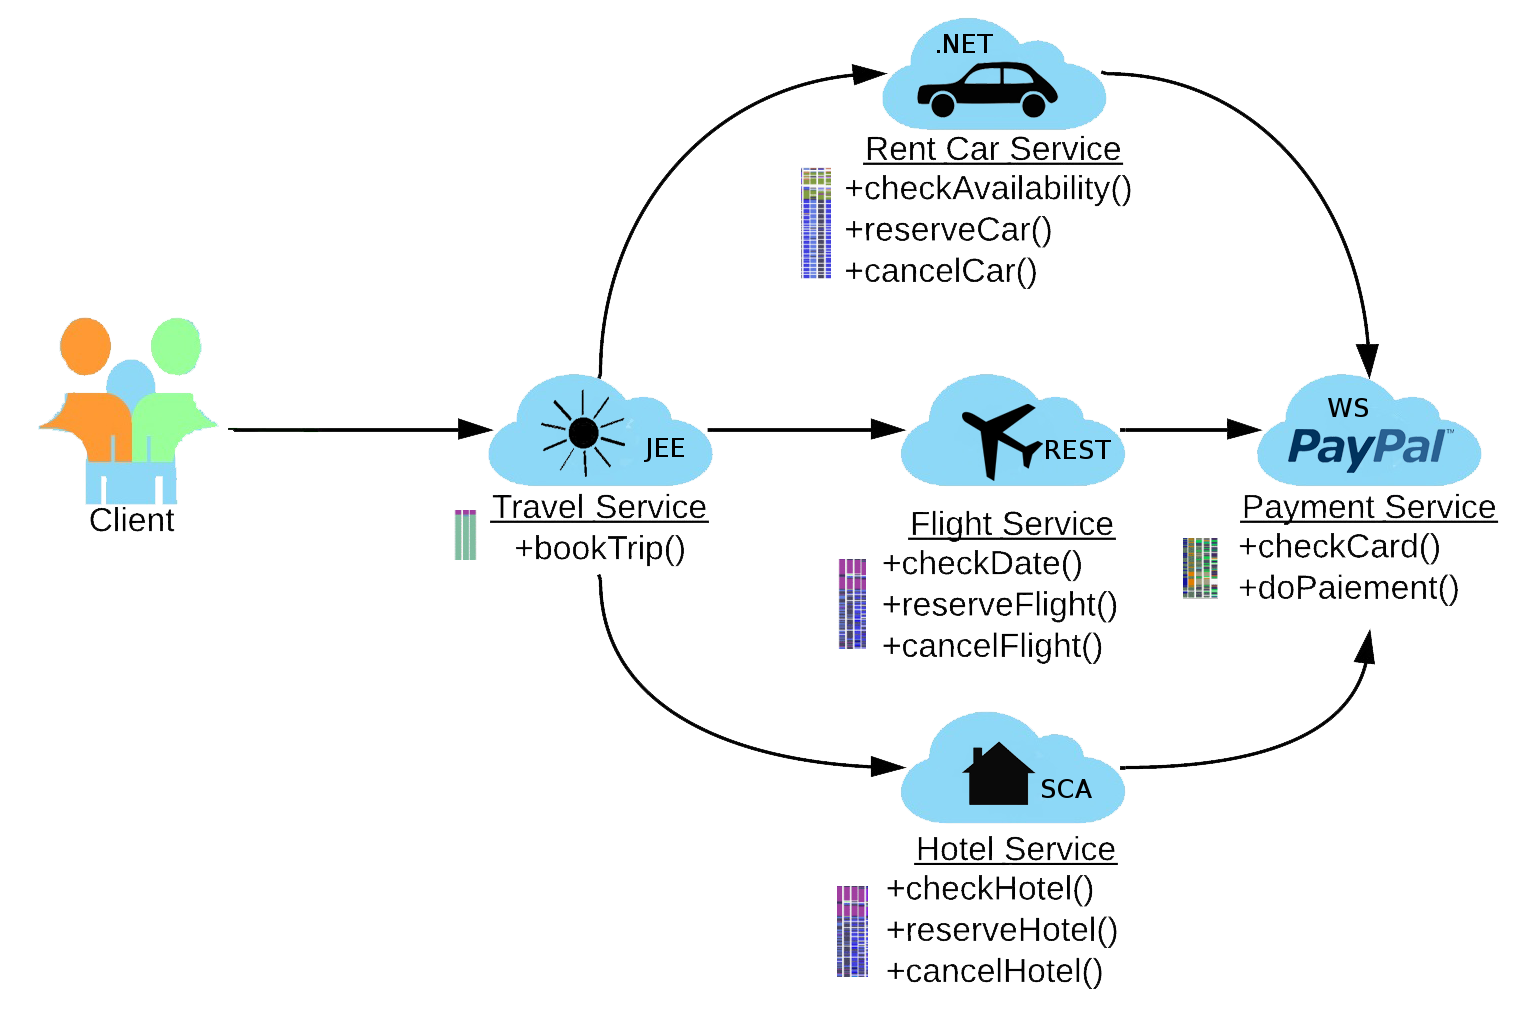
\includegraphics[width=0.8\linewidth]{media/context.png}
\end{figure}

\begin{itemize}
\vspace{-1cm}
\item Uses various technologies
\item Constant evolution may \textbf{degrade} the system $\Rightarrow$ \textbf{Antipatterns}
\item \textbf{SOA Antipatterns} are \textbf{detectable} manifestations
of these degradations \cite{p1}
\end{itemize}
\end{frame}

\begin{frame}
\vspace{-0.2cm}
\frametitle{Context: Two Typical SOA Antipatterns}
\begin{figure}
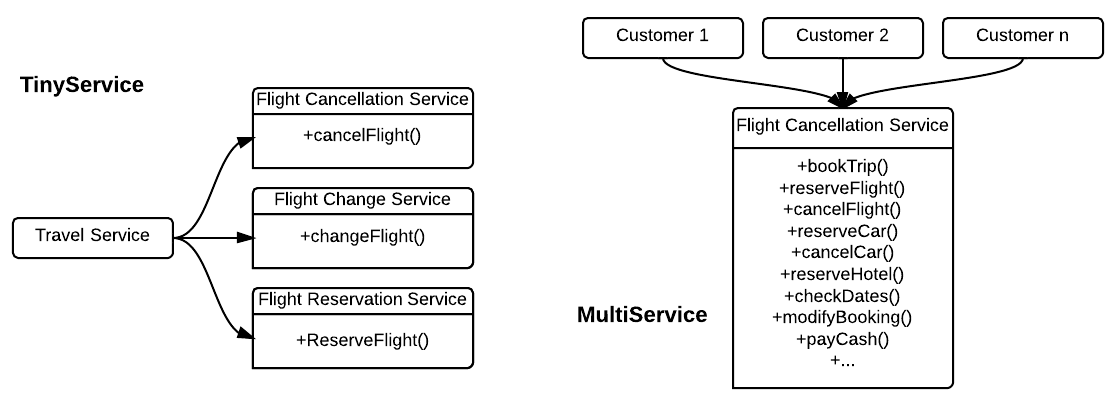
\includegraphics[width=0.8\linewidth]{media/AP.png}
\end{figure}
\vspace{-0.3cm}
\begin{block}{Tiny Service}
Implements \textbf{few methods} that require \textbf{several coupled services} to complete an abstraction \cite{p2}.
\end{block}

\begin{block}{Multi Service}
Implements a \textbf{multitude of methods}, not easily reusable because of \textbf{low cohesion} of methods,  \textbf{often unavailable} due to \textbf{overload} \cite{p2}.
\end{block}

\end{frame}

\begin{frame}
\frametitle{Problem}
\textbf{How can the Design and the Quality of Service Based Systems be enhanced through automatic refactoring ?}
\vspace{0.5cm}
\begin{itemize}
\item Accurately detect antipatterns in SBSs.
\item Reverse-engineer the architecture of SBSs.
\item Refactor the architecture while keeping the same functionalities.
\item Create a better (quality-wise) execution plan.
\end{itemize}

\end{frame}

\begin{frame}
\frametitle{Related Work}
\begin{columns}[c] % The "c" option specifies centered vertical alignment while the "t" option is used for top vertical alignment

\column{.45\textwidth} % Left column and width
\textbf{Quality based Refactoring}
\begin{itemize}
\item \underline{OO Systems}: \hfill \\ Decades of research. FCA, RCA, model transformation, metric based, rule based...
\item \underline{SOA Systems}: \hfill \\ Focus on availability, reliability, cost, response time. \\ Do not deal with software quality
\end{itemize}

\column{.5\textwidth} % Left column and width
\textbf{Service Composition By Planning}
\begin{itemize}
\item Compose stateless services
\item Compose statefull services
\item Compose coordinated asyn-
chronous statefull services
\item Focus on aggregate/orchestrate services
\item Advanced planning techniques and algorithms
\item Actually suggest antipatterns.
\end{itemize}
\end{columns}
\vspace{1.5cm}
\end{frame}

\begin{frame}
\frametitle{SOMAD-R: A different direction}
\begin{itemize}
\item Based on SOMAD, a precise and efficient SBSs antipattern detector
\begin{itemize}
\item Point out antipatterns
\item Provide the architecture of the SUT
\end{itemize}
\item Uses a custom version of the LAMA Planner
\begin{itemize}
\item Evolution of the Fast-Downward planner
\item Prizes winner
\end{itemize}
\item Heuristics that aim to remove antipatterns while conserving the observable behaviour
\begin{itemize}
\item Multiple Orienteering Problem
\end{itemize}
\item Was able to remove antipatterns (3/5) and to improve the performance (32\%) of a small scale system
\end{itemize}
\end{frame}


\begin{frame}
\frametitle{Approach}

\begin{figure}

\includegraphics[width=1\linewidth]{media/approach.png}
\end{figure}
\begin{itemize}
\item Feed SOMAD with execution traces of the SUT + Metrics + AP Specification
\item RE-SOA + Antipatterns
\item Goal extraction from the RE-SOA
\item Re-orchestration of the services through planning under heuristics
\item Produce traces for the new orchestration and send them to SOMAD
\item Loop until a perfect plan is reached or OOT/OOM
\end{itemize}

\end{frame}

\begin{frame}
\frametitle{Approach: Step 1 - SOMAD Extraction}


\begin{columns}[c] 
\column{.45\textwidth} % Left column and width
\textbf{Gathering And Aggregating Traces \cite{p3}}

\begin{figure}
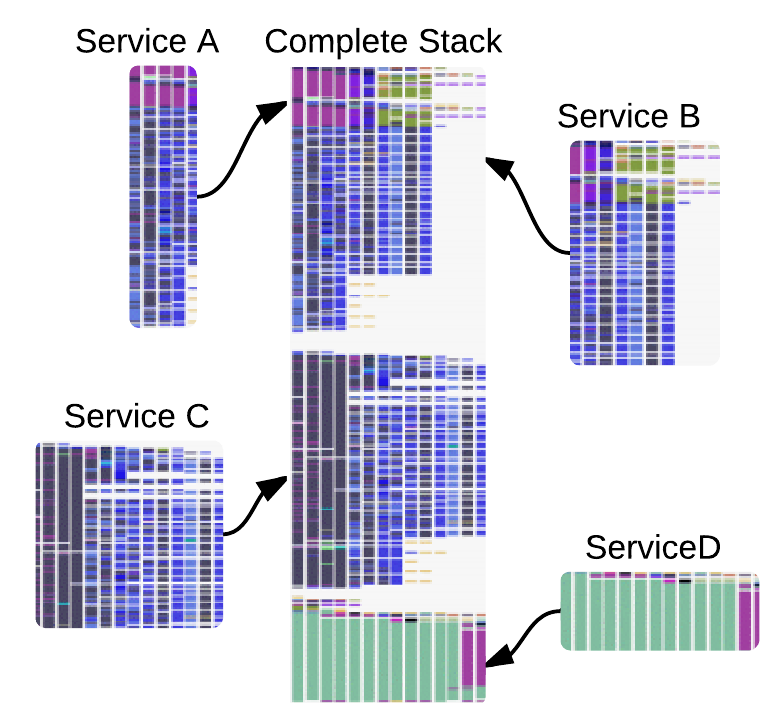
\includegraphics[width=1\linewidth]{media/SOMAD4-1.png}
\end{figure}


\column{.5\textwidth} % Left column and width

\textbf{Extracting SAR \cite{p4}}
\begin{figure}
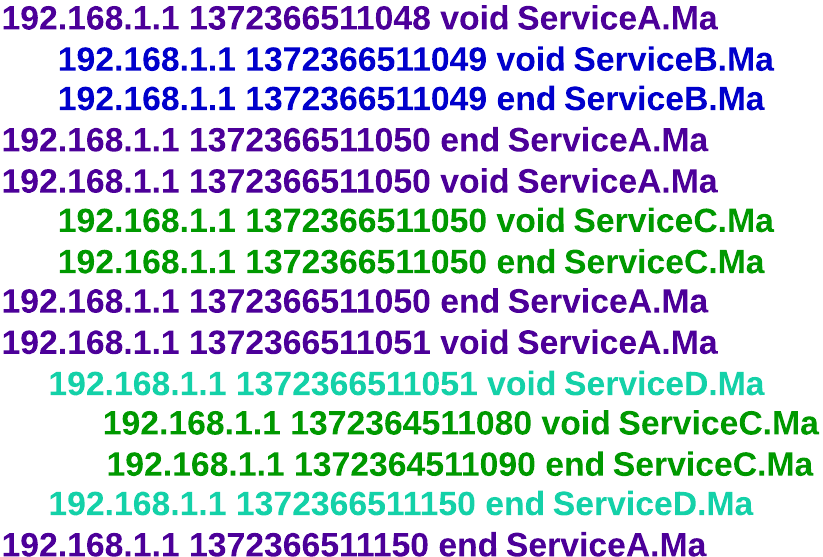
\includegraphics[width=0.6\linewidth]{media/SOMAD4-2.png}
\end{figure}
\begin{center}
\textbf{A $\Rightarrow$ B, A $\Rightarrow$ C, A $\Rightarrow$ D, C}\\
\end{center}
\begin{figure}
\vspace{-0.5cm}
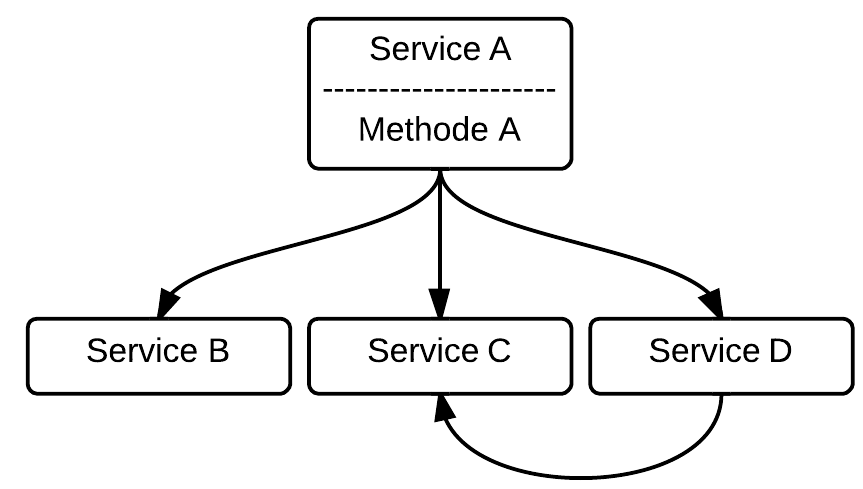
\includegraphics[width=0.6\linewidth]{media/SOMAD4-3.png}
\end{figure}
\end{columns}
\end{frame}

\begin{frame}
\frametitle{Approach: Step 2 - Planning}
\begin{itemize}
\item Automated Planning is a branch of AI
\begin{itemize}
\item Transform an environment on a given state to an environment that satisfies given goal(s)
\item Each action have effect and can require pre-condition 
\end{itemize}
 
\begin{equation}
\sum  = (S, A, E, \gamma)
\end{equation}

\item Where S, A, E represent the states, actions and events, respectively and $\gamma$ represents the state-transition function :

\begin{equation}
\gamma: S * (A \cup E)
\end{equation}
\item The required complexity to solve a planning problem
can be much more than NP-Complete or even undecidable.
\end{itemize}
\end{frame}

\begin{frame}
\frametitle{Approach: Step 2 - Planning}
\begin{itemize}
\item Not always deterministic 
\begin{itemize}
\item Services output can change
overtime
\end{itemize}
\item Dynamic 
\begin{itemize}
\item Services can be added or removed at any time
\end{itemize}
\item The system is not fully observable
\begin{itemize} 
\item Inside logic of services are unknown
\end{itemize}
\item Do not know what are the possible actions as we deduct them from SOMAD
\item Try to construct qualitative plans with a sub-set of the actions
\end{itemize}
\end{frame}

\begin{frame}
\begin{itemize}
\item Each node is a service
\item Contains a set of sub-nodes
accessible only by him and representing its methods
\item Construct the problem based on SOMAD output
\item Cost of initialization / method execution
\end{itemize}
\frametitle{Approach: Step 2 - Planning}
\begin{figure}
    \centering
	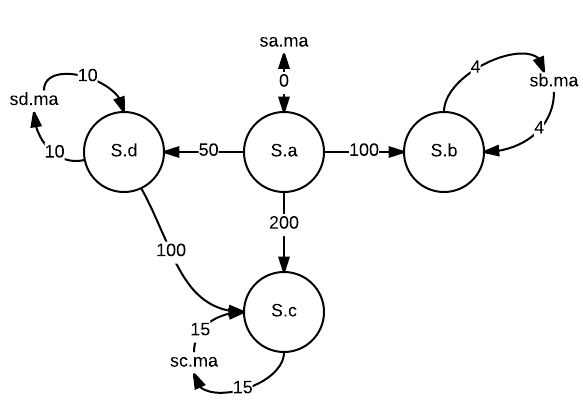
\includegraphics[scale=0.3]{media/orienteering.png}
 	\caption{Orienteering problem.}
    \label{fig:orienteering}
\end{figure}
\end{frame}

\begin{frame}
\frametitle{Approach: Step 2 - Planning}
\begin{figure}
    \centering
	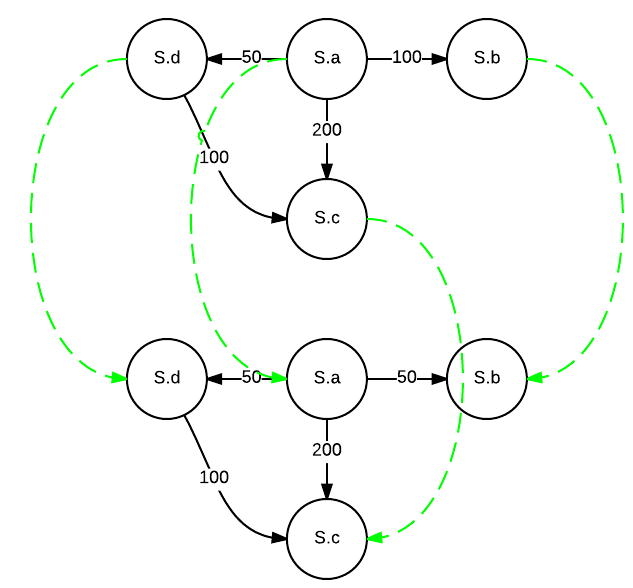
\includegraphics[scale=0.35]{media/multiple_orienteering.png}
 	\caption{Multiple Orienteering problem.}
    \label{fig:multiple_orienteering}
\end{figure}
\end{frame}

\begin{frame}
\frametitle{Approach: Step 2 - Planning}
\begin{itemize}

\item Landmarks
\begin{itemize}
\item Propositional formulas that must be true in every generated plan
\item In order to speed-up the plan generation and
find the shortest solution, LAMA directs its search towards states containing
many true landmarks
\end{itemize}
\item Action costs
\begin{itemize}
\item In classical planning, actions  execute themselves in discrete time
\item LAMA adapts the Landmarks so they use the time and the cost of actions.
\item We use the solution of the multiple orienteering problem from the previous step as a baseline for the cost of actions
\end{itemize}
\item Anytime Search
\begin{itemize}
\item When LAMA reaches a solution to the planning problem, it
continues to search for the best solution by using successive weighted A* graphs.
\end{itemize}
\end{itemize}
\end{frame}

\begin{frame}
\frametitle{Approach: Step 3 - Generation of mockup traces}
\begin{itemize}
\item The output of the planning step is a set of executable actions
\item We don't have any clues on the quality of this plan
\item We generate mockup execution traces based on our current plan
\end{itemize}
\begin{small}
192.168.1.1 1372366511048 in ServiceA.Ma\\
...192.168.1.1 1372366511436 in ServiceD.Ma\\
......192.168.1.1 1372366511536 in ServiceC.Ma\\
......192.168.1.1 1372366511566 out ServiceC.Ma\\
...192.168.1.1 1372366511586 out ServiceD.Ma\\
...192.168.1.1 1372366511686 in ServiceB.Ma\\
...192.168.1.1 1372366511694 out ServiceB.Ma\\
192.168.1.1 1372366511694 out ServiceA.Ma
\end{small}
\begin{itemize}
\item The generated traces are sent back to SOMAD which will assess the quality
of the solution in terms of antipatterns
\end{itemize}

\end{frame}


\begin{frame}
\frametitle{Experimentations}

\begin{itemize}
\item HomeAutomation
\begin{itemize}
\item SCA application for domotic (elderly citizens home)
\item 3.2 KLOC, 13 services, 226 methods, 48 classes
\item 7 predefined uses-cases scenarios
\end{itemize}
\end{itemize}
\begin{figure}
    \centering
	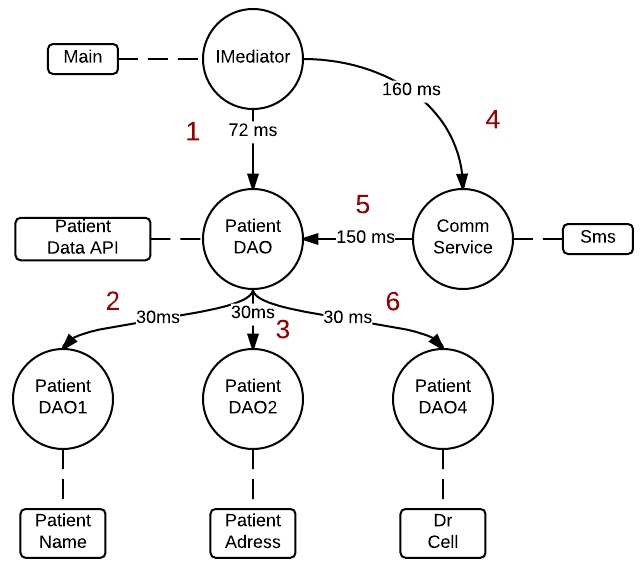
\includegraphics[scale=0.3]{media/scenario1.png}
 	\caption{HomeAutomation scenario: Send patient information to his doctor (original
orchestration).}
    \label{fig:multiple_orienteering}
\end{figure}
\end{frame}

\begin{frame}
\frametitle{Experimentations}

\begin{itemize}
\item Original orchestration
\begin{itemize}
\item 5 different antipatterns
\item Executes in 472ms
\item Multi-Service: IMediator
\item Chatty-Service: PatientDAO and IMediator
\item Knot: PatientDAO
\item BottleNeck: PatientDAO, IMediator
\item Chain Service : IMediator $\rightarrow$ Communicaton Service $\rightarrow$ PatientDAO $\rightarrow$ PatientDAO\{1,2,4\}
\end{itemize}
\item Two different LAMA planners
\begin{itemize}
\item Original greedy heuristics
\item Orienteering problem
\end{itemize}
\end{itemize}
\end{frame}

\begin{frame}
\frametitle{Experimentations}
\begin{itemize}
\item Greedy
orchestration
\end{itemize}
\begin{figure}
    \centering
	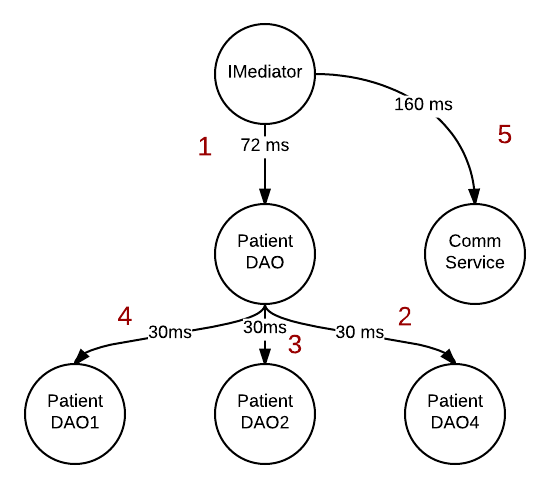
\includegraphics[scale=0.3]{media/scenario2.png}
\end{figure}
\begin{itemize}
\item Removes the Service chain antipattern
\item Executes in 400 ms (-15\%)
\end{itemize}
\end{frame}


\begin{frame}
\frametitle{Experimentations}
\begin{itemize}
\item Orienteering orchestration
\end{itemize}
\begin{figure}
    \centering
	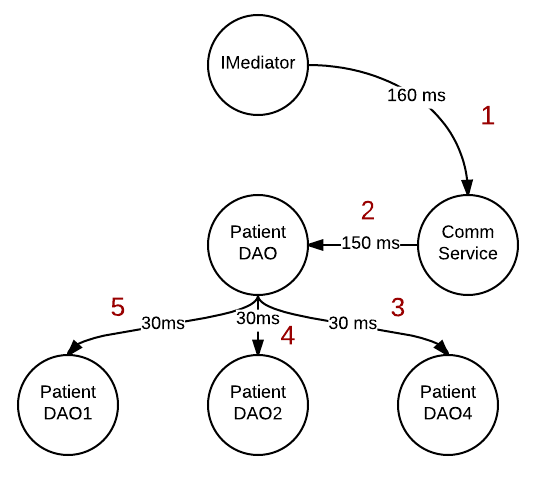
\includegraphics[scale=0.3]{media/scenario3.png}
\end{figure}
\begin{itemize}
\item Removes the Knot, The Bottleneck and the Multiservice
\item Executes in 322 ms (-32\%)
\end{itemize}
\end{frame}

\begin{frame}
\frametitle{Conclusion}
\begin{itemize}
\item Refactor the initial system and
reduce the number of SOA Anitpatterns instances from 5 to 2 without loss any
functionalities
\item Reduce the needed time for its execution by 32\%
\vspace{1cm}
\item Weight SOA antipatterns instead of counting them and
improve our heuristic
\item Real-scale systems
\end{itemize}


\end{frame}


\begin{frame}
\frametitle{References}
\footnotesize{
\begin{thebibliography}{99} % Beamer does not support BibTeX so references must be inserted manually as below
\bibitem[Moha, 2012]{p1} N. Moha, F. Palma, M. Nayrolles et al. (2012)
\newblock Specification and Detection of
SOA Antipatterns
\newblock \emph{ICSOC 2012} 1 -- 16.
\bibitem[Dudney, 2003]{p2} Bill Dudney, Stephen Asbury, Joseph K. Krozak, and Kevin Wittkopf. (2003)
\newblock J2EE AntiPatterns. John Wiley \& Sons Inc
\bibitem[Yousefi, 2011]{p3} A. Yousefi and K. Sartipi,
. (2011)
\newblock Identifying distributed features in SOA by
mining dynamic call trees
\newblock \emph{ICSM 2011} 73 -- 82.
\bibitem[Fournier-Vigier, 2011]{p4} A. Fournier-Viger, R. Nkambou, and V. Tseng. (2011)
\newblock Rulegrowth: mining
sequential rules common to several sequences by pattern-growth
\newblock \emph{SAC 2011} 956 -- 961.

\end{thebibliography}
}
\end{frame}


%------------------------------------------------

\begin{frame}
\Huge{\centerline{QUESTIONS?}}
\end{frame}

%----------------------------------------------------------------------------------------

\end{document} 
